% Algoritmy: https://docs.google.com/document/d/1cDg8dV4Rso5sAE2gYkBPsJ8a_dMLqA8MHRR1ZvceWZM/edit#heading=h.7z19cc4fgwy4
%TODO: Our results indi-cate that network models used by many previous works might produce results
%that are off by an order of magnitude in comparison to a more realistic model. Additionally, we
%show that certain implementation details of scheduling algorithms which
%are often neglected can have a large effect on the scheduler’s performance, and they
%should thus be described in great detail to enable proper evaluation.

Task scheduling is one of the most important responsibilities of a task runtime in terms of
performance, because the quality of the generated schedule has a large effect on the total makespan
of the task graph execution and also on the achieved hardware utilization of worker nodes. It is
crucial for the scheduler to be able to distribute the tasks amongst all available worker nodes to
achieve as much parallelization as possible, without the induced network communication and task
management becoming a bottleneck. Unfortunately, optimal task scheduling is a very difficult
problem, which is NP-hard even in the simplest cases~\cite{Ullman1975}, and there is thus no
single scheduling algorithm that could quickly provide an optimal schedule for an arbitrary task
graph.

There are many factors that affect the execution properties of task graphs and that pose some form
of a challenge to task schedulers. The execution environment (e.g.\ a distributed cluster) can have
varying amounts of nodes with heterogeneous hardware resources, and complex network topologies that
can have a non-trivial effect on the latency and bandwidth of messages sent between the workers and
the scheduler, and thus in turn also on the overall performance of the task graph execution. Task
graphs can be structured arbitrarily, with large amounts of different kinds of tasks with diverse
execution characteristics and resource requirements.

Furthermore, task graph execution might not be deterministic, and the scheduler has to work with
incomplete information and react to events that dynamically occur during task execution and that
cannot be fully predicted before the task graph has started executing. The communication network
can be congested because of unrelated computations running concurrently on the cluster, tasks can
also be slowed down by congested hardware resources that can be highly non-trivial to model (e.g.\
NUMA effects), and they can also sometimes fail unpredictably and must be re-executed. Even the
duration of each task, which is perhaps the most crucial property of a task coveted by the
scheduler, is usually not known beforehand, and the most the scheduler knows about is either an
estimate from the task graph author or a running average based on historical executions of similar
tasks, both of which can be inaccurate.

In theory, all these factors should be taken into account by task scheduling algorithms. In
practice, it is infeasible to have a completely accurate model of the entire cluster, operating
system, task implementations, networking topology etc. Therefore, task schedulers omit some of
these factors to provide reasonable runtime performance. They rely on various heuristics and make
different trade-offs that make them better suited for specific types of task graphs and execution
environments. These heuristics can suffer from non-obvious edge cases that produce bad quality
schedules or from low runtime efficiency, which can in turn erase any speedup gained from producing
a higher quality schedule.

For HPC use-cases, the performance and quality of task scheduling is even more important, since the
scale and heterogeneity of task graphs used in HPC provides a challenge for the scheduler. HPC
clusters also tend to provide advanced network topologies with low latency and high
bandwidth~\cite{dragonfly,slimfly}, which offer the scheduler more leeway to create sophisticated
schedules leveraging large amounts of network communication, which would otherwise be infeasible on
clusters with slower networks.

To better understand the behaviour and performance of various scheduling algorithms, we have
performed an extensive analysis of several task scheduling algorithms in
\emph{Analysis of workflow schedulers in simulated distributed environments}~\cite{estee}. The two main contributions of this work are as
follows:
\begin{enumerate}
	\item We have created an extensible, open-source simulator of task graph execution, which allows users to
	      easily implement their own scheduling algorithms and compare them, while taking into account
	      various factors that affect task scheduling.
	\item We have benchmarked several task schedulers from existing literature under various conditions,
	      including factors affecting scheduling that have not been explored so far, like the minimum delay
	      between invoking the scheduler or the amount of knowledge about task durations available to the
	      scheduler, and evaluated the suitability of the individual algorithms for various types of task
	      graphs. All parts of the benchmark suite in an open and reproducible form. This includes the task
	      graphs, all source code for the schedulers and the simulation environment and also all benchmark
	      scripts.
\end{enumerate}

Various descriptions of schedulers, task graphs and other parts of the simulator and the benchmark
configuration used in this chapter were adapted from our publication~\cite{estee}.

\workshare{I have collaborated on this work with Ada Böhm and Vojtěch Cima, we have all contributed to it equally. Source code contribution statistics for
\estee{} can be found on GitHub\footnoteurl{https://github.com/it4innovations/estee/graphs/contributors}.}

\section{Task graph simulator}
\label{sec:estee-simulator}
To analyse scheduling algorithms, some form of an environment for executing task has to be used.
One possibility would be to use an actual distributed cluster, and implement multiple schedulers
into an existing task runtime. However, this approach can be quite expensive, both computationally
(executing a large amount of task graphs with various configurations would consume a lot of cluster
computational time) and implementation-wise (adapting existing runtimes to different scheduling
algorithms is challenging). Therefore, task graph scheduling surveys tend to use some form of a
simulated environment, which simulates selected properties of a distributed cluster, and allows
comparing the performance of multiple scheduling algorithms (or other factors of a task runtime)
with smaller accuracy, but at a fraction of the  cost.

Many task scheduler surveys have been published over the years~\cite{hlfet1974, kwok1998benchmarking, hagras2003static, sinnen2005, wang2018list}, yet it is
difficult to reproduce and extend these results without having access to the exact source code used
to implement the schedulers and the simulation environment used in these surveys. As we will show
in the following chapter, the performance of scheduling algorithms can be highly affected by
seemingly trivial implementation details, and having access only to a high-level textual
description or pseudocode of a scheduling algorithm doesn't guarantee that it will be possible to
reproduce it independently with the same performance characteristics. This makes it challenging to
compare results between different simulation environments.

Apart from the environments used in existing surveys, there are also more general task simulation
environments. DAGSim~\cite{dagsim} offers a framework for comparing scheduling algorithms,
and compares the performance of a few algorithms, but doesn't provide its implementation, which
makes it difficult to reproduce or extend its results. SimDAG~\cite{simdag} is a task
graph simulator focused on HPC use-cases built on top of the SimGrid~\cite{simgrid}
framework. It allows relatively simple implementation of new task scheduling algorithms, however it
does not support any task resource requirements (e.g.\ the number of used CPU cores).

In addition to simply comparing the performance of different schedulers, our goal was also to test
two factors that affect scheduling, which we haven't seen explored in detail in existing works.
Namely, we wanted to examine the effects of MSD (\emph{minimal scheduling delay}), the delay between two
invocations of the scheduler and \emph{information mode}, the amount of knowledge of task durations
that is available to the scheduler. These factors will be described in detail in the following
section. The existing simulation environments that we have evaluated did not have support for these
factors, and it would be non-trivial to add support for them.

To summarize, our goal was to have a simulation environment that would be open-source, to provide
full reproducibility, would support basic task resource requirements and would enable us to examine
the two mentioned factors that affect scheduling. To fulfill these goals, we have implemented a new
task graph simulation framework called \estee{}. It is an \mbox{MIT-licensed}
open-source tool\footnoteurl{https://github.com/it4innovations/estee} written in Python that provides an experimentation testbed
for task runtime and scheduler developers and researchers. It is quite flexible, and can be used to
define a cluster of workers, connect them together using a configurable network model, implement a
custom scheduling algorithm and test its performance on arbitrary task graphs, with support for
specifying required CPU core counts for individual tasks. At the same time, it comes
``battery-included'', and contains baseline implementations of several task schedulers from
existing literature and also a task graph generator that can be used to generate randomized graphs
with properties similar to real-world task graphs.

\subsection{Architecture}
Figure~\ref{fig:estee-architecture} shows the architecture of \estee{}. The core of the
tool is the Simulator component, which uses discrete event simulation to simulate the execution of
a task graph. It manages task lifetime, queries the Scheduler component for task-to-worker
assignments (schedules) and then assigns the tasks to their corresponding workers. The Worker
component then simulates task execution, and also uses the provided network model to simulate
exchanges of data (task outputs) between the individual workers in the simulated cluster.

\begin{figure}
	\centering
	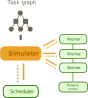
\includegraphics[scale=0.35]{estee/estee-architecture}
	\caption{\estee{} architecture}
	\label{fig:estee-architecture}
\end{figure}

\estee{} provides abstract interfaces for the task scheduler, the worker and the
network model (which simulates network communication and congestion). Users can thus easily provide
their own implementations of these interfaces, and in turn override both the behavior of the
scheduler and of the cluster and its network topology.

One of our goals for \estee{} was to make it very easy to write new scheduling
algorithms and make the scheduler approachable for other researchers that might want to experiment
with task schedulers. That was also one of the motivations why we decided to create
\estee{} in Python, which facilitates experimentation. Listing~\ref{lst:estee-example}
shows an example of a task graph simulation that demonstrates the simplicity of defining task graph
simulation using\estee{}. The output of the simulation is both the makespan (the
duration it took to execute the task graph) and also a detailed trace that can be used to visualize
the individual task-to-worker assignments and task execution time spans.

\begin{listing}
	\caption{Simple task graph simulation example using \estee{}}
	\label{lst:estee-example}
	\begin{minted}[fontsize=\small]{python}
# Create task graph containing 3 tasks
# (each task runs for 1s and requires 1 CPU)
#
#     t0
#     | (50MB output)
#    / \
#  t1   t2
tg = TaskGraph()
t0 = tg.new_task(duration=1, cpus=1, output_size=50)
t1 = tg.new_task(duration=1, cpus=1)
t1.add_input(t0)
t2 = tg.new_task(duration=1, cpus=1)
t2.add_input(t0)

# Create a task scheduler
scheduler = BlevelGtScheduler()

# Define cluster with 2 workers (1 CPU each)
workers = [Worker(cpus=1) for _ in range(2)]

# Define MaxMinFlow network model (100MB/s bandwidth)
netmodel = MaxMinFlowNetModel(bandwidth=100)

# Run simulation, returns the makespan in seconds
simulator = Simulator(tg, workers, scheduler, netmodel, trace=True)
makespan = simulator.run()
print(f"Task graph execution makespan = {makespan}s")
\end{minted}
\end{listing}

\estee{} supports general task graphs represented by a directed acyclic graph (DAG).
Each task has an associated duration, and can contain multiple outputs (data objects), each with an
associated size. It can also specify how many cores does it require, to model the common
requirement of executing multithreaded functions and programs on modern HPC machines. The used
model of a task graph corresponds precisely to the task graph definition contained in
Chapter~\ref{ch:taskgraphs}.

\subsection{Communication model}
Some previous scheduler surveys assume that the time to transfer a data object from one worker to
another depends merely on the size of the data object, and not on other factors, such as current
network utilization or interference~\cite{tang2010list,yao2013task,wang2018list,kwok1996dynamic}. This is an unrealistic assumption, as
the latency and bandwidth of actual computer networks is affected (amongst other things) by other
communication happening concurrently on the same network. Moreover, a real worker implementation
would download more than a single data object simultaneously, which further affects the transfer
durations, because the worker's bandwidth will be shared by multiple network tranfers. We will use
the term \emph{communication model} and \emph{network model} interchangeably in this chapter.

We provide a more realistic network model that simulates full-duplex communication between workers,
where the total (data object) upload and download bandwidth of each worker is limited. The sharing
of bandwidth between worker connections is modeled by the
\emph{max-min fairness model}~\cite{bertsekas_1992}. Max-min fairness provides a bandwidth allocation for
each worker. If an allocation of any participant is increased, then we necessarily have to decrease
the allocation of some other participant with an equal or smaller allocation. When a data object
transfer starts or finishes, the data flow between workers is recomputed immediately, thus we
neglect the fact that it may take some time for the bandwidth to fully saturate.

%TODO: odkomentovat?
%This model is not as accurate as e.g.\ packet-level simulation implemented in some other
%simulators~\cite{simgrid}, but it is a notable improvement over the naive model.

To provide a baseline that corresponds to the naive model described above, which has been used in
several previous works, \estee{} also implements a \emph{simple} network model.

It is possible to choose an arbitrary network bandwidth amount for a given simulation for any used
networking model.

\subsection{Scheduler parameters}
%TODO: odstranit konec této  věty?
\estee{} implements support for two parameters that can affect scheduler performance,
and which we have not seen examined in detail in existing literature:
\begin{description}
	\item[Minimal scheduling delay] Non-trivial schedulers create task assignments continuously during task graph execution, based on
		the current worker load and task completion times. That means that they are not invoked only once,
		but rather the task runtime invokes them repeatedly, to ask them to produce assignments for tasks
		that are (or soon will be) ready to be executed at any given point in time.

		It then becomes an important for a task runtime to decide when exactly should it invoke the
		scheduler. It could try to make a scheduling decision every time a task is finished; however, in
		practice there is often an upper bound on the number of scheduler invocations per second. It might
		be introduced artificially, to reduce the scheduling overhead, or it might be caused by a software
		or hardware limitation (e.g.\ messages containing task updates cannot be received more often).
		Furthermore, creating a new schedule after each task status change might not be optimal. The
		runtime can also accumulate changes for a short time period, and then provide the scheduler with a
		batch of status updates. While this increases the latency of task assignments, it can give the
		scheduler more context to work with, when it decides how it should assign tasks to workers.

		To test our hypothesis that the scheduler invocation rate can affect its performance, we introduce
		a parameter called \emph{Minimal scheduling delay (MSD)}, which forces a minimal delay between two scheduler
		invocations, i.e.\ the scheduler cannot be invoked again before the at least MSD time units have
		elapsed since its previous invocation.
	\item[Information mode] Many existing task scheduler descriptions assume that the duration of each task (and the size of
		each data object) is known in advance. However, this assumption is very seldom upheld when
		executing real-world task graphs. Tasks are usually specified using arbitrary functions or binary
		invocations, and it can be quite difficult to estimate their duration up front. Task runtimes thus
		have to work with completely missing information about task durations, depend on potentially
		imprecise user estimates, or calculate their own estimates based on historical task execution data.
		Task benchmarks usually use simulated task durations, which are provided to the scheduler. However,
		this might not realistically represent the scheduler's behavior for actual task graphs, for which
		we usually do not know task durations precisely.

		We use a parameter called \emph{Information mode (imode)}, which controls the amount of knowledge the
		scheduler has of the duration of tasks. It can be set to one of the following values:
		\begin{description}
			\item[\emph{exact}] The scheduler has access to the exact duration of each task and the exact size of each data object
				in the whole task graph.
			\item[\emph{user}] The scheduler has access to user-defined estimations for each task in the task graph. These
				estimations are sampled from a random distribution that corresponds to a specific kind of task
				within the workflow. For example, in a task graph that performs three kinds of tasks (e.g.\
				preprocessing, computation and postprocessing), each kind of task would have its own distribution.
				We have categorized the tasks of task graphs that we have used for scheduler benchmarks described
				in Section~\ref{sec:estee-benchmarks} manually, to simulate a user that has some knowledge of the task
				graph that they are trying to compute and is able to provide some estimate of task durations and
				data object sizes.
			\item[\emph{mean}] The scheduler has only access to the mean duration of all tasks and the mean size of all data
				objects in the executed task graph. This simulates a situation where a similar task graph is
				executed repeatedly, and thus there is at least some aggregated information about the task
				properties available from an earlier run.
		\end{description}
		Another possible mode to consider could be to not provide the scheduler with any task durations nor
		data object sizes in advance. This behaviour would in fact correspond quite closely to a real-world
		execution of a task graph, where we usually do not know these task properties a priori. However, it
		is challenging to use this approach when benchmarking schedulers. Scheduler implementations are
		typically described with the assumption that task durations are known, and the scheduling
		algorithms are often fundamentally based on calculations that make use of them.

		If we took away this information, it would make many schedulers very sensitive to an initial
		estimate of the durations and sizes (and the ratio between them, which influences decisions whether
		to move data objects between workers to enable more parallelization). This estimate strongly
		influences the behavior of schedulers, and if task durations would be completely unknown, the
		behavior of different schedulers could converge and be heavily affected by the estimate.

		It is also unclear how to even compute such an estimate, which would have to be chosen almost
		arbitrarily. Therefore, we propose to use the \emph{mean} mode instead of not providing
		the scheduler with any information. This assumes that even if the scheduler knows nothing in
		advance, it could always monitor the durations and sizes of finished tasks gradually and such
		monitored values would converge to the mean. In practice, this would take some time, while in our
		environment the schedulers know about the mean in advance. Nevertheless, as was already mentioned,
		we can often get a reasonable estimate of the mean durations based on previous executions of
		similar workflows.
\end{description}

%TODO: uncomment?
%\subsection{Worker inner scheduler}
%Since each worker has to keep track of its running tasks, manage resources, and
%handle data object transfers, it becomes quite complex. In practice, the global
%scheduler cannot micromanage each worker because this approach could not scale
%to a larger number of workers. Therefore, we model a situation where each
%worker has its own inner scheduler. We call it \emph{w-scheduler} and we
%reserve the word ``scheduler'' for the global scheduler that assigns tasks to
%workers.
%
%The w-scheduler is not a subject of study in this work, hence we are going to
%fix one particular worker scheduler and execute all experiments with it.
%The implementation is inspired by the worker implementation used in
%HyperLoom~\citep{hyperloom} and Rain. It is described in Appendix~A.

\subsection{Schedulers}
There are many task scheduling approaches, and an enormous amount of various task scheduling
algorithms. We have implemented a set of task schedulers that are representatives of several common
scheduling approaches, inspired by a list of schedulers from a survey performed by Wang and
Sinnen~\cite{wang2018list}. We have included several representatives of the simplest and perhaps
most common list-scheduling approach, but also schedulers that use work-stealing or genetic
algorithms.

List-scheduling is an intuitive approach where the scheduler sorts tasks (into a list) based on
some priority criteria, and then repeatedly chooses the task with the highest priority, and assigns
it to a worker (which is selected by another heuristic).

Below is a list of schedulers that we have implemented and benchmarked\footnote{The labels of the individual schedulers correspond to labels used in charts that will be presented
in a Section~\ref{sec:estee-benchmarks}.}:
\noindent\textbf{blevel}\quad Highest Level First with Estimated
Times~\cite{hlfet1974} (HLFET) is a foundational list-based scheduling algorithm that prioritizes
tasks based on their \emph{b-level}. B-level of a task is the length of the longest path
from the task to any leaf task (in our case the length of the path is computed using durations of
tasks, without taking data object sizes into account). The tasks are scheduled in a decreasing
order based on their b-level.

\noindent\textbf{tlevel}\quad
Smallest Co-levels First with Estimated Times~\cite{kwok1999static} is similar to HLFET, with the
exception that the priority value computed for each task (which is called \emph{t-level}
here) is computed as the length of the longest path from any source task to the given task. This
value corresponds to the earliest time that the task can start. The tasks are scheduled in an
increasing order based on their t-level.

\noindent\textbf{dls}\quad
Dynamic Level Scheduling~\cite{sih1993compile} calculates a dynamic level for each task-worker
pair. It is equal to the static b-level lessened by the earliest time that the task can start on a
given worker (considering necessary data transfers). In each scheduling step, the task-worker pair
that maximizes this value is selected.

\noindent\textbf{mcp}\quad
The Modified Critical Path~\cite{wu1990hypertool} scheduler calculates the ALAP
(as-late-as-possible) time for each task. This corresponds to the latest time the task can start
without increasing the total schedule makespan. The tasks are then ordered in ascending order based
on this value, and scheduled to the worker that allows their earliest execution.

\noindent\textbf{etf}\quad
The ETF (Earliest Time First) scheduler~\cite{hwang1989scheduling} selects the task-worker pair that
can start at the earliest time at each scheduling step. Ties are broken by a higher b-level
precomputed at the start of task graph execution.

\noindent\textbf{genetic}\quad
This scheduler uses a genetic algorithm to schedule tasks to workers, using the mutation and
crossover operators described in~\cite{omara2009genetic}. Only valid schedules are considered, if no
valid schedule can be found within a reasonable amount of iterations, a random schedule is
generated instead.

\noindent\textbf{ws}\quad
This is an implementation of a simple work-stealing algorithm. The default policy is that each task
that is ready to be executed (when all its dependencies are already computed) is always assigned to
a worker where it can be started with a minimal transfer cost. The scheduler then continuously
monitors the load of workers. When a worker starts to starve (and thus doesn't have enough tasks to
compute), then a portion of tasks assigned to other workers is rescheduled to the starving worker.

In addition to these schedulers, we have also implemented several naive schedulers, which serve as
a baseline for scheduler comparisons.

\noindent\textbf{single}\quad
This scheduler simply assigns all tasks to a single worker (it selects the worker with the most
cores). The resulting schedule never induces any data transfers between workers, and doesn't take
advantage of any parallelism between workers.

\noindent\textbf{random}\quad
This scheduler simply assigns each task to a random worker using a PRNG (pseudo-random number
generation) engine.

We have tried to implement the mentioned list-based schedulers (\emph{blevel}, \emph{tlevel},
\emph{dls}, \emph{mcp}, \emph{etf}) as closely as possible to their original description.
These list-based algorithms mostly focus on selecting the next task to schedule, but an important
question (that comes up during their implementation) is to what worker should the selected task
be scheduled. The algorithm description often mention assigning the task to a worker that allows
the earliest start time of the task. While that is surely a reasonable heuristic, it is not clear
how exactly should such a worker be found, because the exact earliest start time often cannot be
determined precisely in advance, since its calculation might encompass network transfers whose
duration is uncertain by nature. This seemingly simple implementation detail is crucial for
impementing the scheduler, and it should be included in the description of all scheduling algorithms.

\estee{} implementations of these schedulers use a simple estimation of the earliest start time, which
is based on the currently executing and already scheduled tasks of a worker, and an estimated
network transfer cost based on uncontended network bandwidth (in other words, the \emph{simple}
network model is used for the scheduler's estimation of the network transfer cost).

In order to test our hypothesis that the worker selection is quite important and affects the
scheduler's behavior, we have also created extended versions of the \emph{blevel},
\emph{tlevel} and \emph{mcp} schedulers. These modified versions use a worker selection heuristic
called ``greedy transfer``. We have not applied this heuristic to other list-based schedulers, where
it would fundamentally change their behavior.

%TODO: reword this? better differentiate between the naive heuristic and greedy-transfer?
The greedy transfer heuristic assigns the selected task to a worker that has a sufficient number of
free cores on which the task may be executed and that requires the minimal data transfer (sum over all
sizes of data objects that have to be transferred to that worker). It also adds support for clusters
where some machines have a different number of cores than others. When a task $t$ that needs $c$ cores cannot be scheduled
because of an insufficient number of free cores, the list scheduling continues
by taking another task in the list instead of waiting for more free cores. This
task will only consider workers that have less than $c$ cores. This allows to
schedule more tasks while it does not modify the priority of tasks because $t$
cannot be scheduled on such workers anyway. Note that when all workers have the
same number of cores, the behavior is identical to ordinary list scheduling.

\subsection{Task graphs}
To facilitate task scheduler experiments, \estee{} contains a task graph generator, which is able to
generate parametrized instances of various categories of task graphs. Graphs from each category can
be generated using several parameters that affect their resulting size and shape. To increase the
variability of the graphs, properties like task durations or data object sizes are sampled from
a normal distribution. Below is a description of the three categories of task graphs that can be
generated:

%TODO: explain fork-join?
\vspace{1mm}\noindent\textbf{elementary}\quad This category contains trivial graph shapes, such as tasks
with no dependencies or simple fork-join graphs. These graphs can test the behavior of scheduler
heuristics on basic task graph building blocks that frequently form parts of larger workflows. Examples
of these graphs can be seen in Figure~\ref{fig:estee-elementary-shapes}.

\vspace{1mm}\noindent\textbf{irw}\quad This generator creates graphs that are inspired by real-world
workflows, such as machine learning cross-validations or map-reduce computations.

\vspace{1mm}\noindent\textbf{pegasus}\quad This category is derived from graphs created by the Synthetic
Workflow Generators~\cite{pegasusgraphs}. The generated graphs correspond to the \emph{montage},
\emph{cybershake}, \emph{epigenomics}, \emph{ligo} and \emph{sipht} Pegasus workflows.
The graphs have been extended with additional properties required for testing information modes
(notably expected task durations and data object sizes for the \emph{user} information mode).

\section{Task scheduler benchmarks}
\label{sec:estee-benchmarks}
We have performed an extensive analysis of the performance of several task scheduling algorithms on
various task graphs using the \estee{} simulator. The aim of the analysis was to
explore the behavior of various schedulers in a complex simulation environment. In addition to
comparing the schedulers amongst each other, we also wanted to test how does their performance differ
between various communication models and scheduler parameters. The benchmarking environment and
all configurations, input datasets, results and charts are freely available as reproducible
artifacts~\cite{estee_results}.

Note that since the used simulation environment is focused on simulating different task graph
schedules and network transfers, and it does not model the actual execution of the scheduler nor
the task runtime in a cycle-accurate way, the term \emph{scheduler performance} refers to the simulated
makespan of task graphs executed using schedules provided by the given scheduler. Our goal is thus
to compare how quickly would a given task graph be fully computed on a cluster (and a network
model) while being scheduled by different scheduling algorithms, while also taking into account the
mentioned scheduler parameters.

\subsection{Benchmark configuration}
This section describes the cluster, scheduler and task graph configurations that we have used for our
benchmarks.

\begin{description}
	\item[Task graphs] The \estee{} graph generators were used to generate a collection of task graphs
	that were used in the benchmarks. The properties of all used graphs are summarized in Table~\ref{tab:estee-graph-properties}.
	The generated task graph dataset is available as a reproducible artifact~\cite{estee_graphs}.
	\item[Schedulers] We have benchmarked all schedulers described in Section~\ref{sec:estee-simulator}.
	Schedulers that use the greedy transfer heuristic are labeled with a \emph{-gt} suffix in benchmark
	results.
	\item[Scheduler parameters] To evaluate the effect of minimal scheduling delay, we have used a baseline
	value of zero, where the scheduler is invoked immediately after any task status update, and then
	a delay of 0.1, 0.4, 1.6 and 6.4 seconds. In the cases where MSD is non-zero, we have also added
	a 50 milliseconds delay before sending the scheduler decision to workers, to simulate the time
	taken by the scheduler to produce the schedule. For experiments that do not focus on MSD, we
	always use an MSD of 0.1 seconds and the 50 milliseconds computation delay.
	To evaluate information modes, we have used the \emph{exact}, \emph{user} and \emph{mean} imodes.
	For experiments that do not focus on imodes, we always use the \emph{exact} mode.
	\item[Network models] The simple (labeled \emph{simple}) and max-min (labeled \emph{max-min}) network
	models were used, with bandwidth speeds ranging from 32 MiB/s to 8 GiB/s. For experiments that do
	not focus on the network model (e.g.\ when imodes are compared), we always use the \emph{max-min}
	network model.
	\item[Clusters] We have used the following five cluster (worker) configurations
	(where $w \times c$ means that the cluster has $w$ workers and each worker has $c$ cores):  8$\times$4,
		16$\times$4, 32$\times$4, 16$\times$8, 32$\times$16.
\end{description}

%TODO: fix cut task graph
\begin{figure}
	\centering
	\begin{subfigure}{.2\textwidth}
		\centering
		\includegraphics[width=.8\textwidth]{imgs/estee/shapes/plain}
		\caption{}
		\label{fig:tg-plain}
	\end{subfigure}%
	\begin{subfigure}{.2\textwidth}
		\centering
		\includegraphics[width=.8\linewidth]{imgs/estee/shapes/fork}
		\caption{}
		\label{fig:tg-fork}
	\end{subfigure}
	\begin{subfigure}{.2\textwidth}
		\centering
		
\includegraphics[width=.8\linewidth]{imgs/estee/shapes/fork2}
		\caption{}
		\label{fig:tg-fork2}
	\end{subfigure}
	\begin{subfigure}{.2\textwidth}
		\centering
		
\includegraphics[width=.8\linewidth]{imgs/estee/shapes/v}
		\caption{}
		\label{fig:tg-v}
	\end{subfigure}
	\\
	\begin{subfigure}{.2\textwidth}
		\centering
		
\includegraphics[width=.8\linewidth]{imgs/estee/shapes/w}
		\caption{}
		\label{fig:tg-w}
	\end{subfigure}
	\begin{subfigure}{.2\textwidth}
		\centering
		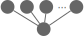
\includegraphics[width=.8\linewidth]{imgs/estee/shapes/merge}
		\caption{}
		\label{fig:tg-merge}
	\end{subfigure}
	\begin{subfigure}{.2\textwidth}
		\centering
		
\includegraphics[width=.8\linewidth]{imgs/estee/shapes/merge-triplets}
		\caption{}
		\label{fig:tg-merge-triplets}
	\end{subfigure}
	\begin{subfigure}{.2\textwidth}
		\centering
		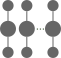
\includegraphics[width=.8\linewidth]{imgs/estee/shapes/triplets}
		\caption{}
		\label{fig:tg-triplets}
	\end{subfigure}
	\\
	\begin{subfigure}{.2\textwidth}
		\centering
		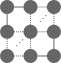
\includegraphics[width=.8\linewidth]{imgs/estee/shapes/grid}
		\caption{}
		\label{fig:tg-grid}
	\end{subfigure}
	\begin{subfigure}{.2\textwidth}
		\centering
		\includegraphics[width=.8\linewidth]{imgs/estee/shapes/splitters}
		\caption{}
		\label{fig:tg-splitters}
	\end{subfigure}
	\begin{subfigure}{.2\textwidth}
		\centering
		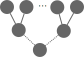
\includegraphics[width=.8\linewidth]{imgs/estee/shapes/conflux}
		\caption{}
		\label{fig:tg-conflux}
	\end{subfigure}
	\begin{subfigure}{.2\textwidth}
		\centering
		
\includegraphics[width=.8\linewidth]{imgs/estee/shapes/fern}
		\caption{}
		\label{fig:tg-fern}
	\end{subfigure}

	\caption{Task graph shapes in the \emph{elementary} data set}
	\label{fig:estee-elementary-shapes}
\end{figure}

\begin{table}
	\caption{Scheduler benchmark task graph properties}
	\centering
	\label{tab:estee-graph-properties}
	\begin{tabular}{l|lrrrr|T}
		\toprule
		Graph & D &   \#T &     \#O & TS &   LP & \normalsize{Description} \\
		\midrule
		plain1n &   e &  380 &      0 &    0.00 &    1 &   Independent tasks;
		normally distributed durations (Fig.~\ref{fig:tg-plain}) \\
		plain1e &   e &  380 &      0 &    0.00 &    1 &    Independent tasks;
		exponentially distributed durations (Fig.~\ref{fig:tg-plain}) \\
		plain1cpus &   e &  380 &      0 &    0.00 &    1 &  Independent tasks with
		varying core requirements (Fig.~\ref{fig:tg-plain}) \\
		triplets &   e &  330 &    220 &   17.19 &    3 & Task triplets; middle
		task requires 4 cores (Fig.~\ref{fig:tg-triplets}) \\
		merge\_neighb. &   e &  214 &    107 &   10.36 &    2 & Merge of adjacent
		task pairs (Fig.~\ref{fig:tg-w}) \\
		merge\_triplets &   e &  148 &    111 &   10.77 &    2 & Merge of task
		triplets (Fig.~\ref{fig:tg-merge-triplets}) \\
		merge\_sm-big &   e &  240 &    160 &    7.74 &    2 &  Merge of two
		results (0.5 MiB and 100 MiB data objects) (Fig.~\ref{fig:tg-v}) \\
		fork1 &   e &  300 &    100 &    9.77 &    2 &      Tasks with a pair of
		consumers each consuming the same output (Fig.~\ref{fig:tg-fork})  \\
		fork2 &   e &  300 &    200 &   19.53 &    2 &      Tasks with a pair of
		consumers each consuming different output (Fig.~\ref{fig:tg-fork2}) \\
		bigmerge &   e &  321 &    320 &   31.25 &    2 &    Merge of a large
		number of tasks (variant of Fig.~\ref{fig:tg-merge}) \\
		duration\_stairs &   e &  380 &      0 &    0.00 &    1 &    Independent
		tasks; task durations range from 1 to 190 s (Fig.~\ref{fig:tg-plain}) \\
		size\_stairs &   e &  191 &    190 &   17.53 &    2 &  1 producer 190
		outputs / 190 consumers; sizes range from 1 to 190 MiB \\
		splitters &   e &  255 &    255 &   32.25 &    8 &  Binary tree of
		splitting tasks (Fig.~\ref{fig:tg-splitters}) \\
		conflux &   e &  255 &    255 &   31.88 &    8 &    Merging task pairs
		(inverse of \emph{splitters}) (Fig.~\ref{fig:tg-conflux}) \\
		grid &   e &  361 &    361 &   45.12 &   37 & Tasks organized in a 2D grid
		(i.e. \emph{splitters} followed by \emph{conflux}) (Fig.~\ref{fig:tg-grid})
		\\
		fern &   e &  401 &    401 &   11.11 &  201 &       Long task sequence with
		side tasks (Fig.~\ref{fig:tg-fern}) \\ \hline
		gridcat &   i &  401 &    401 &  115.71 &    4 & Merge of pairs of 300 MiB
		files  \\
		crossv &   i &   94 &     90 &    8.52 &    5 &  Cross validation \\
		crossvx &   i &  200 &    200 &   32.66 &    5 & Several instances of cross
		validation \\
		fastcrossv &   i &   94 &     90 &    8.52 &    5 & Same as \emph{crossv}
		but tasks are $50\times$ shorter \\
		mapreduce &   i &  321 &  25760 &  439.06 &    3 & Map-reduce pattern \\
		nestedcrossv &   i &  266 &    270 &   28.41 &    8 & Nested cross
		validation \\ \hline
		montage &   p &   77 &    150 &    0.21 &    6 &        Montage workflow
		from Pegasus \\
		cybershake &   p &  104 &    106 &    0.84 &    4 &        Cybershake
		workflow from Pegasus \\
		epigenomics &   p &  204 &    305 &    1.36 &    8 &        Epigenomics
		workflow from Pegasus \\
		ligo &   p &  186 &    186 &    0.11 &    6 &        Ligo workflow from
		Pegasus \\
		sipht &   p &   64 &    136 &    0.12 &    5 &        Sipht workflow from
		Pegasus \\
		\bottomrule
	\end{tabular}\\
	\vspace{2mm}
	D = Dataset (e = elementary, i = irw, p = pegasus);
	\#T = Number of tasks; \#O = Number of outputs;
	TS = Sum of all output object sizes (GiB);
	LP = longest oriented path in the graph
\end{table}

\subsection{Evaluation}
%EXPAND: show Estee charts, describe the results in more detail

%%%%%%%%%%%%%%%%%%%%%%%%%%%%%%%%%%%==
Our analysis has shown that despite its simplicity, the foundational HLFET
algorithm~\cite{hlfet1974} produces high quality schedules in various scenarios and should
thus serve as a good baseline scheduler for task runtimes. We have also found out that even a
completely random scheduler can be competitive with other scheduling approaches for certain task
graphs and cluster configurations.

%During our attempts to implement various scheduling algorithms, we have also realized that the
%descriptions of many task scheduling algorithms in existing literature is incomplete. More
%specifically, seemingly inconsequential implementation details that are often missing from the
%algorithm's description can have a very large effect on the final performance of the scheduler,
%which makes it difficult to precisely reproduce and compare the performance of the existing
%algorithms.

% List-Scheduling versus Cluster-Scheduling
% - simple schedulers are surprisingly competitive
